\documentclass[11pt,letterpaper]{article}
\usepackage[margin=1.02in]{geometry}
\usepackage[T1]{fontenc}
\usepackage{lmodern,microtype}
\usepackage{amsmath,amssymb,amsthm,mathtools}
\usepackage{booktabs,longtable,array}
\usepackage{graphicx,xcolor}
\usepackage{pgfplots}
\pgfplotsset{compat=1.18}
\usepackage[colorlinks=true,urlcolor=blue!55!black,linkcolor=blue!45!black,citecolor=blue!45!black]{hyperref}
\usepackage[capitalize,noabbrev]{cleveref}
\setlength{\parskip}{4pt}
\setlength{\parindent}{0pt}
\newtheorem{conjecture}{Conjecture}[section]
\newtheorem{theorem}[conjecture]{Theorem}
\newtheorem{proposition}[conjecture]{Proposition}
\newtheorem{lemma}[conjecture]{Lemma}
\newtheorem{corollary}[conjecture]{Corollary}
\theoremstyle{remark}
\newtheorem{remark}[conjecture]{Remark}
\newcommand{\GPF}{P^{+}}
\newcommand{\rad}{\operatorname{rad}}
\newcommand{\iiota}{\iota}
\newcommand{\Om}{\omega}
\newcommand{\PsiSmooth}{\Psi}
\newcommand{\PC}{\mathrm{PC}}
\title{\bfseries Prime-Support Dilution in Consecutive Integer Products\\[4pt]
\large Conjectures, finite tests, unconditional sparsity, and possible routes to a uniform proof}
\author{Research working note developed in human--AI mathematical discussion}
\date{22 October 2026\\Version 3: Result 012 review\\Private research working draft}
\begin{document}
\maketitle
\begin{abstract}
For $N=m(m+1)$, let $\Om(N)$ be its number of distinct prime factors and let
$\iiota(N)=\pi(\GPF(N))$ be the index of its greatest prime factor. We propose
\emph{prime-support dilution}: $\Om(m(m+1))/\iiota(m(m+1))\to0$ as
$m\to\infty$, and the more speculative bound
$\Om(m(m+1))\le\iiota(m(m+1))^{1/2+\varepsilon}$ for every
$\varepsilon>0$ and sufficiently large $m$.
Both statements are stronger than finiteness of prime-complete consecutive
products (OEIS A141399). We give a new, self-contained derivation of an
\emph{unconditional} sparse-exception statement: for each fixed $\delta>0$,
the number of $m\le X$ for which at least a $\delta$-fraction of the initial
prime indices occur is $X^{o(1)}$. We also give an elementary unbounded lower
bound for the maximal support function. Conditional on the strong
Lagarias--Soundararajan $xyz$ conjecture, an exponent-$2/3$ upper bound follows
for the maximal number of prime divisors of consecutive $p_r$-smooth integers.
A comparison with Erd\H{o}s Problem 368 shows that its conjectural lower bound
$P^+(m(m+1))\gg(\log m)^2$ would imply our square-root variant.
We examine OpenAI's September 2026 Result 012, which claims a natural-density
joint Dickman theorem for consecutive integers, and carefully distinguish its
fixed power-scale conclusions from the uniform logarithmic-scale estimates
needed here. New exhaustive finite enumeration through $r=20$ gives the exact values of that
maximum and supplies a reproducibility check against two OEIS sequences.
The small-order data do \emph{not} yet provide convincing evidence for an
asymptotic exponent $1/2$. We separate rigorous results, conditional
implications, heuristic arguments, and the unproved step needed for a proof
independent of $xyz$.
\end{abstract}

\section{Motivation and exact notation}
Let $p_1=2<p_2=3<\cdots$ denote the primes, and set
\[
  P_r=p_r^\#=\prod_{i=1}^r p_i,\quad
  \Om(n)=\#\{p:p\mid n\},\quad
  \iiota(n)=\pi(\GPF(n)),\quad n>1.
\]
Here $p_r$-smooth means \emph{no prime factor greater than $p_r$}.
In particular, \emph{19-smooth is $p_8$-smooth}, not $p_{19}$-smooth.
For $m\ge1$ put
\[
 s(m)=\Om(m(m+1)),\qquad r(m)=\iiota(m(m+1)),\qquad
 D(m)=\frac{s(m)}{r(m)},\qquad \Delta(m)=r(m)-s(m).
\]
The value $D(m)$ lies in $(0,1]$. We call $D(m)$ the \emph{prime-support
fraction}. A product $m(m+1)$ is prime-complete (PC) precisely when
\[
\rad(m(m+1))=P_{r(m)} \quad\Longleftrightarrow\quad D(m)=1.
\]
The known values of $m$ satisfying this equation form OEIS A141399
\cite{A141399}; the largest known is $633555$. Its global maximality is
unproved. The present proposal changes the focus from the absence of
\emph{complete} support to the asymptotic \emph{fraction} of support attained.

For each $r\ge1$ define the finite St\o rmer set and its two extremal
statistics:
\begin{align*}
\mathcal S_r&=\{m\ge1:\GPF(m(m+1))\le p_r\},\\
U_r&=\max\mathcal S_r=\mathrm{A002072}(r),\\
W(r)&=\max_{m\in\mathcal S_r}\Om(m(m+1)).
\end{align*}
St\o rmer's theorem guarantees that $\mathcal S_r$ is finite for fixed $r$
\cite{Stormer,Lehmer}. Note that $W(r)$ is \emph{not} the maximum $\Om$
in a primorial interval. It maximizes over \emph{all consecutive
$p_r$-smooth pairs}, regardless of their size.

\section{A hierarchy of conjectures}
\begin{conjecture}[Prime-support dilution]\label{conj:dilution}
\[
\boxed{\displaystyle \lim_{m\to\infty}D(m)=0.}
\]
Equivalently, the fraction of missing primes below the greatest prime factor
satisfies $\Delta(m)/r(m)\to1$.
\end{conjecture}

\begin{conjecture}[Power-saving dilution]\label{conj:power}
There exists $\eta>0$ such that, for all sufficiently large $m$,
\[
\Om(m(m+1))\le \iiota(m(m+1))^{1-\eta}.
\]
\end{conjecture}

\begin{conjecture}[Square-root dilution; speculative]\label{conj:sqrt}
For every $\varepsilon>0$, for all sufficiently large $m$,
\[
\boxed{\Om(m(m+1))\le\iiota(m(m+1))^{1/2+\varepsilon}.}
\]
\end{conjecture}

\begin{proposition}[Equivalent maximal formulation]\label{prop:equiv}
Conjecture~\ref{conj:dilution} is equivalent to
\[
\boxed{W(r)=o(r).}
\]
Likewise Conjecture~\ref{conj:sqrt} is equivalent to
$W(r)\le r^{1/2+o(1)}$.
\end{proposition}
\begin{proof}
For $m\in\mathcal S_r$, $\Om(m(m+1))\le W(r)$, and setting
$r=r(m)$ gives the easy implication from $W(r)/r\to0$ to
$D(m)\to0$. For the converse, fix $\varepsilon>0$; the dilution
hypothesis gives an $M$ such that $s(m)<\varepsilon r(m)$ for $m>M$.
When $m\le M$, $s(m)$ is bounded independently of $r$. Thus for all
$m\in\mathcal S_r$,
\[
 s(m)\le\max\{\max_{m\le M}s(m),\varepsilon r\},
\]
and $W(r)/r\le\varepsilon+o(1)$. For the power bound, the finitely many
$m\le M_\varepsilon$ are again harmless, while $r(m)\le r$.
\end{proof}

The hierarchy is
\[
\begin{gathered}
\text{square-root dilution}\Longrightarrow\text{power-saving dilution}
\Longrightarrow\text{dilution}\\
\Longrightarrow\text{eventual non-PC}
\Longrightarrow\text{A141399 finite}.
\end{gathered}
\]
The final implication needs care: $D(m)\to0$ ensures that $D(m)=1$
occurs only finitely often, but the converse is not known. In
particular, disproving the square-root law would not by itself disprove
A141399 termination.

\section{What is provable unconditionally?}
\subsection{High-support pairs must be logarithmically smooth}
\begin{lemma}[Critical smoothness obstruction]\label{lem:logsmooth}
Fix $0<\delta\le1$. Every sufficiently large $m$ with $D(m)\ge\delta$
satisfies
\[
\boxed{\GPF(m(m+1))\le\left(\frac{2}{\delta}+o(1)\right)\log(m+1).}
\]
The $o(1)$ is interpreted along sequences with $r(m)\to\infty$;
for bounded $r(m)$ the bound is automatic for large $m$.
\end{lemma}
\begin{proof}
Write $r=r(m)$ and $s=s(m)\ge\delta r$. The $s$ distinct primes
of $m(m+1)$ have product at least $P_s$. Thus
\[
2\log(m+1)>\log(m(m+1))\ge \log P_s=\vartheta(p_s).
\]
The prime number theorem yields, for fixed $\delta>0$ and $r\to\infty$,
\[
\vartheta(p_s)\ge\vartheta(p_{\lceil\delta r\rceil})
 =(\delta+o(1))p_r.
\]
Rearranging proves the result. If $r$ stays bounded, $p_r$ is bounded
and the displayed inequality holds trivially for sufficiently large $m$.
\end{proof}

This lemma is a concrete, unconditional consequence of the support
fraction condition: a hypothetical infinite family retaining a fixed
positive fraction of prime indices would force infinitely many
consecutive pairs whose largest prime factor is at most a constant
times the logarithm of their size. That is the $xyz$-critical scale,
not a generic smoothness condition.

\subsection{An unconditional subpolynomial exceptional set}
Define
\[
E_\delta(X)=\#\{1\le m\le X:D(m)\ge\delta\}.
\]
\begin{theorem}[Sparsity of non-dilute support]\label{thm:sparse}
For every fixed $\delta>0$,
\[
\boxed{E_\delta(X)=X^{o(1)}\qquad (X\to\infty).}
\]
More quantitatively, with a constant depending on $\delta$,
\[
E_\delta(X)\le
\exp\left(O_\delta\!\left(
\frac{\log X\,\log\log\log X}{\log\log X}
\right)\right)
\]
for sufficiently large $X$.
\end{theorem}
\begin{proof}
By Lemma~\ref{lem:logsmooth}, there is $C_\delta>0$ such that every
sufficiently large $m$ counted by $E_\delta(X)$ is
$C_\delta\log X$-smooth. Hence, for fixed $\delta$,
\[
E_\delta(X)\le O_\delta(1)+\PsiSmooth(X,C_\delta\log X),
\]
where $\PsiSmooth(X,y)$ counts positive $y$-smooth integers at most $X$.
For $X$ large put $y=C_\delta\log X$ and
$\sigma=1/\log\log X>0$. Rankin's elementary inequality gives
\[
\PsiSmooth(X,y)
\le X^\sigma\prod_{p\le y}(1-p^{-\sigma})^{-1}.
\]
Since $p\ge2$ and $1-2^{-\sigma}\asymp\sigma$, the logarithm of the
Euler product is at most
\[
\pi(y)\log\frac{1}{1-2^{-\sigma}}
=O_\delta\left(
\frac{\log X}{\log\log X}\log\log\log X\right).
\]
Moreover, $\sigma\log X=\log X/\log\log X$. The asserted bound
follows on exponentiating.
\end{proof}

\begin{remark}[What the theorem does \emph{not} say]
For any $\delta>0$ the exceptional set has natural density zero and,
in fact, grows more slowly than $X^\varepsilon$ for every fixed
$\varepsilon>0$. Yet $X^{o(1)}$ may still tend to infinity. The theorem
does \emph{not} prove eventual absence of exceptions, dilution for every
$m$, or the finiteness of A141399. The existential uniform problem is
precisely where the existing methods lose control.
\end{remark}

\subsection{An unconditional lower bound on the smooth-pair maximum}
\begin{proposition}[Unbounded support capacity]\label{prop:lower}
As $r\to\infty$,
\[
\boxed{W(r)\ge(1+o(1))\frac{\log r}{\log\log r}.}
\]
\end{proposition}
\begin{proof}
Let $k$ be maximal with $P_k+1\le p_r$. The pair
$(m,m+1)=(P_k,P_k+1)$ is $p_r$-smooth, since every prime factor of
either member is at most $P_k+1\le p_r$. Its members are coprime;
therefore the product has at least $k+1$ distinct prime factors.
Consequently $W(r)\ge k+1$. From $\log P_k=\vartheta(p_k)
\sim k\log k$ and $p_r\sim r\log r$, maximality implies
$k=(1+o(1))\log r/\log\log r$.
\end{proof}
This lower bound leaves an enormous interval between the known
unconditional growth and the proposed square-root upper law.

\section{Finite enumeration: direct evidence and its limits}
We performed an exhaustive enumeration of every consecutive
$p_r$-smooth pair for $1\le r\le20$, using the maximum starting
values $U_r$ tabulated by OEIS A002072 \cite{A002072}.
The counts were independently cross-checked against OEIS A002071
\cite{A002071}. Enumerating all $p_{20}$-smooth positive integers at
most $U_{20}=119089041053696$, checking whether the successor is
$p_{20}$-smooth, and recording the distinct-prime support gives
$4,839$ consecutive pairs. The source code supplied with this note
implements this exact integer enumeration; its output is supplied
as a separate CSV file. The enumeration uses the published endpoints:
it does not independently reprove the St\o rmer certificates determining
those endpoints.

\begin{table}[htbp]
\centering
\small
\begin{tabular}{@{}rrrrrr@{}}
\toprule
$r$ & $p_r$ & $\#\mathcal S_r$ & $W(r)$ & $W(r)/r$ & example $m$ attaining $W(r)$\\
\midrule
1&2&1&1&1.000&1\\
2&3&4&2&1.000&3\\
3&5&10&3&1.000&5\\
4&7&23&4&1.000&35\\
5&11&40&5&1.000&539\\
6&13&68&6&1.000&1715\\
7&17&108&7&1.000&12375\\
8&19&167&8&1.000&633555\\
9&23&241&8&0.889&52325\\
10&29&345&9&0.900&2697695\\
11&31&482&10&0.909&3897165\\
12&37&653&10&0.833&6770555\\
13&41&869&11&0.846&30944913\\
14&43&1153&12&0.857&658831250\\
15&47&1502&13&0.867&1777331555\\
16&53&1930&13&0.813&1777331555\\
17&59&2454&14&0.824&1284729638049\\
18&61&3106&14&0.778&1284729638049\\
19&67&3896&15&0.789&5163068910\\
20&71&4839&15&0.750&5163068910\\
\bottomrule
\end{tabular}
\caption{Exhaustive smooth-neighbor support maxima for $r\le20$.
The final column provides one witness, not necessarily the
largest witness, of the maximum $W(r)$. The pair counts reproduce
A002071; the cutoffs $U_r$ are from A002072.}
\label{tab:data}
\end{table}

\begin{figure}[htbp]
\centering
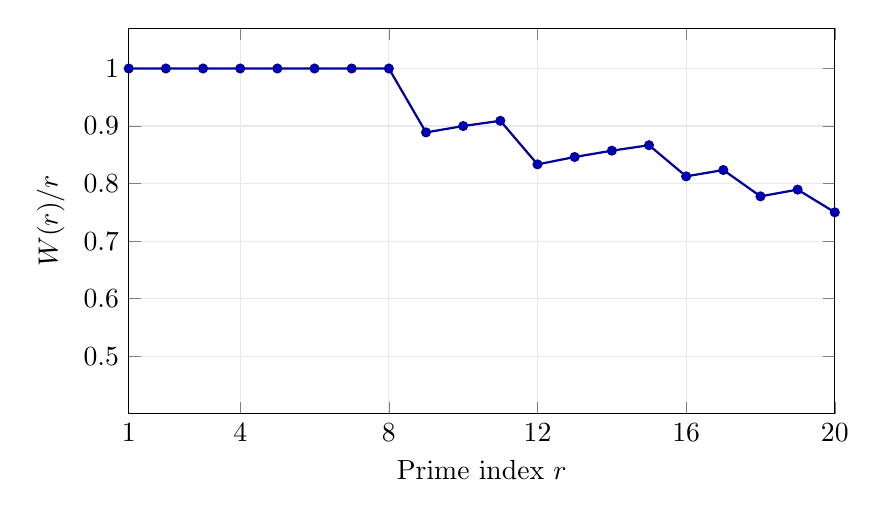
\begin{tikzpicture}
\begin{axis}[
 width=.87\textwidth,height=2.55in,
 xmin=1,xmax=20,ymin=.4,ymax=1.07,
 xlabel={Prime index $r$},ylabel={$W(r)/r$},
 xtick={1,4,8,12,16,20},ytick={.5,.6,.7,.8,.9,1},
 grid=major,grid style={draw=gray!17},
 mark options={scale=.7},
 ]
 \addplot+[thick,mark=*,color=blue!60!black] coordinates {
 (1,1)(2,1)(3,1)(4,1)(5,1)(6,1)(7,1)(8,1)
 (9,.888889)(10,.9)(11,.909091)(12,.833333)(13,.846154)
 (14,.857143)(15,.866667)(16,.8125)(17,.823529)(18,.777778)
 (19,.789474)(20,.75)};
\end{axis}
\end{tikzpicture}
\caption{Finite maximal support fraction. The range is too small
to identify an asymptotic exponent; conspicuous upward jumps remain.}
\end{figure}

These calculations support the observation that \emph{full} support
stops appearing after $r=8$ over the tested range, but do not yet
support a quantitative square-root exponent. Indeed,
$W(20)/20=0.75$, much greater than $20^{-1/2}\approx0.224$;
the conjecture allows non-asymptotic constants and a remote
threshold, so this is not a contradiction, but it is a warning against
overinterpreting the data.

An individual pair may display far more dramatic dilution than the
worst-case maximum. Three exactly factored examples are
\begin{align*}
 m=633555 &: \quad (s,r)=(8,8),\quad D=1,\\
 m=10333245 &: \quad (s,r)=(10,548),\quad D\approx0.01825,\\
 m=715041747420 &: \quad (s,r)=(15,1243236),\quad D\approx0.00001207.
\end{align*}
For the second pair, the new prime factors are $2789$ and $3947$;
for the third, $19540397$ is the largest prime factor. These examples
illustrate the mechanism but are \emph{not representative samples}
and cannot establish an eventual bound for all $m$.


\section{Literature review and a classical conjectural source of the square-root law}\label{sec:lit}
\subsection{Erd\H{o}s Problem 368: the decisive prior-art connection}
Put $F(m)=P^+(m(m+1))$. Erd\H{o}s's long-standing Problem 368 asks
how small $F(m)$ can be and, in particular, records the conjectural
uniform lower bound $F(m)\gg(\log m)^2$; it also records Erd\H{o}s's
complementary expectation that $F(m)<(\log m)^{2+\varepsilon}$
infinitely often, for each $\varepsilon>0$ \cite{Erdos368,Erdos1976}.
The lower-bound statement is not known unconditionally.

\begin{theorem}[Conditional on the conjectured Erd\H{o}s lower bound]
\label{thm:erdos}
If there is a constant $c>0$ such that
$F(m)\ge c(\log m)^2$ for all sufficiently large $m$, then
\[
\omega(m(m+1))\le\iota(m(m+1))^{1/2+o(1)},
\qquad W(r)\le r^{1/2+o(1)}.
\]
In particular, the prime-support dilution conjecture and finiteness
of A141399 follow.
\end{theorem}
\begin{proof}
Let $y=F(m)=p_r$. The assumed bound gives
$\log m\ll\sqrt y$. Since $m(m+1)<(m+1)^2$,
\[
 s=\omega(m(m+1))\le\frac{\log(m(m+1))}{\log 2}
 \ll\sqrt y.
\]
As $r\to\infty$, $y=p_r=r^{1+o(1)}$ by the prime number
theorem, proving $s\le r^{1/2+o(1)}$. For the maximum $W(r)$,
apply the same inequality to each $m\in\mathcal S_r$;
small $m$ contribute bounded $s$, while in the remaining range
$\iota(m(m+1))\le r$. The conclusion follows.
\end{proof}

\begin{proposition}[General power threshold]\label{prop:powthresh}
If for some fixed $\alpha>1$ one has
$F(m)\ge(\log m)^{\alpha-o(1)}$ as $m\to\infty$, then
\[
 \omega(m(m+1))\le\iota(m(m+1))^{1/\alpha+o(1)};
 \qquad W(r)\le r^{1/\alpha+o(1)}.
\]
Consequently any such exponent $\alpha>1$ implies power-saving
dilution and eventual absence of prime-complete products.
\end{proposition}
\begin{proof}
Use $\log m\le F(m)^{1/\alpha+o(1)}$, the elementary
bound $\omega(m(m+1))\ll\log(m+1)$, and
$F(m)=p_{r(m)}=r(m)^{1+o(1)}$. The finite-small-$m$ argument
from Theorem~\ref{thm:erdos} gives the uniform maximum statement.
\end{proof}

This positions our square-root conjecture as a proposed consequence
of a classical, more informative conjecture about the actual size of
the greatest prime factor. The two conjectures are \emph{not} asserted
to be equivalent: small prime support can occur for reasons other
than an unusually large greatest prime factor.

\subsection{The uniform smooth-neighbor ceiling is an equivalent extremal problem}
The sufficient condition proposed in \S\ref{eq:heighttarget},
$\log U_r=o(p_r)$, has an exact reformulation.
\begin{proposition}[Uniform-height/large-factor equivalence]
\label{prop:equivalence}
The following two assertions are equivalent:
\begin{align*}
&\log U_r=o(p_r) \quad (r\to\infty),\\
&\frac{F(m)}{\log m}\longrightarrow\infty \quad(m\to\infty).
\end{align*}
\end{proposition}
\begin{proof}
For a given $m$ set $r=\pi(F(m))$. Then $m\le U_r$, and
$r\to\infty$ with $m$ by fixed-$S$ St\o rmer finiteness.
Hence $\log m/F(m)\le\log U_r/p_r\to0$.
Conversely, $U_r\to\infty$ as $r\to\infty$ (for instance,
$U_r\ge p_r-1$). Put $m=U_r$. Then $F(m)\le p_r$, so
$\log U_r/p_r\le\log U_r/F(U_r)\to0$.
\end{proof}

This equivalence makes a concrete weaker target visible:
$F(m)/\log m\to\infty$ already implies full dilution, though
it does not imply the proposed $1/2$ exponent. A fixed power
saving $F(m)\ge(\log m)^{1+\eta}$ is stronger and yields
power-saving dilution. Erd\H{o}s's quadratic-logarithm conjecture
is stronger still.

\subsection{What is established without abc or xyz?}
The Erd\H{o}s Problems survey records P\'olya's theorem
$F(m)\to\infty$, Mahler's bound $F(m)\gg\log\log m$,
and the later improvement of Pasten \cite{Erdos368,Pasten2024}.
Specifically, Corollary 1.5 of Pasten's 2024 paper gives a lower
bound for the greatest prime factor of $xy(x+y)$, for coprime
positive integers $x<y$. Putting $(x,y)=(1,m)$ yields
\[
 F(m)\gg\frac{(\log\log m)^2}{\log\log\log m}.
\]
This is still very far from $F(m)/\log m\to\infty$.
Pasten's argument combines linear forms in logarithms with
modular and Shimura-curve methods; it is a relevant source for
our elliptic-geometry branch, but it does not furnish the desired
uniform conclusion. His September 2026 follow-up improves a
bound for $n^2+1$, \emph{not} directly the bound for $m(m+1)$
\cite{Pasten2026}; these two polynomial problems must not be conflated.

\subsection{Smooth blocks and distribution results: what they do and do not imply}
Balog and Wooley proved that for any $\varepsilon>0$ there exist
infinitely many increasingly long blocks of consecutive integers
of size roughly $m$ whose prime factors do not exceed $m^\varepsilon$
\cite{BalogWooley}. This does not contradict our conjecture:
the function $m^\varepsilon$ is much larger than any fixed
power of $\log m$.

Work of Ter\"av\"ainen on logarithmic averages, and later work
of Tao--Ter\"av\"ainen and others, investigates joint distributions
of $P^+(m)$ and $P^+(m+1)$ in regimes where the smoothness bound
is a fixed positive power of $m$ \cite{Teravainen2018,TaoTeravainen2019,Wang2021}.
These results substantially inform independence heuristics, but their
asymptotic ranges do not authorize an independence assumption for
$y=(\log m)^C$.

\subsection{OpenAI Result 012: joint Dickman law for consecutive integers}
\label{subsec:result012}
An OpenAI preprint dated September 24, 2026, entitled
\emph{The joint Dickman law for consecutive integers}, appears as
\emph{Result 012: Independent largest prime factors of consecutive
integers} in the October 2026 mathematics release
\cite{OpenAI2026Dickman,OpenAIMathRepository}. The manuscript claims the
following ordinary-natural-density limit. For every fixed pair
$0<a,b<1$,
\begin{equation}\label{eq:joint-dickman}
\lim_{X\to\infty}\frac{1}{X}\#\Big\{2\le m\le X:
\GPF(m)\le m^a,\quad\GPF(m+1)\le m^b\Big\}
=\rho(1/a)\rho(1/b),
\end{equation}
where $\rho$ is the Dickman function. It also claims that each of
$\GPF(m)<\GPF(m+1)$ and $\GPF(m)>\GPF(m+1)$ holds for a set of
natural density $1/2$. These assertions address the Erd\H{o}s--Pomerance
joint-distribution problem (catalogued as Erd\H{o}s Problem 928) and the
ordering problem (Problem 371), respectively
\cite{OpenAI2026Dickman,Erdos928Review}.

\paragraph{Status and formal verification.}
The repository advertises a Lean formalization covering the joint
ordinary-density law and the two ordering statements, rather than all
84 pages of the manuscript. The visible comparator challenge
\texttt{JointDickman.lean} is a statement template: its theorem bodies
contain \texttt{sorry}, which must \emph{not} be mistaken for a completed
proof. A separate solution module is reported, and an independent
October 2026 statement-and-build audit reports successful type checking
without \texttt{sorry} and with the expected foundational axioms
\cite{OpenAILeanScope,Erdos928Review}. We have checked the public
statement, scope descriptions, and this audit, but have \emph{not}
independently replayed its Lean build or refereed the manuscript. We
therefore describe the theorem here as a released, formally reported
result, not as an independently audited theorem of this note.

\paragraph{Relevance and the quantifier obstruction.}
Taking $a=b=\alpha$ in \eqref{eq:joint-dickman} predicts, for
every \emph{fixed} $0<\alpha<1$, a positive proportion
$\rho(1/\alpha)^2$ of pairs for which both integers are
$m^\alpha$-smooth. This is an important confirmation of smooth-neighbor
correlations at fixed power scales. But our extremal problem needs a
bound on \emph{every} sufficiently large $m$, or on the last
consecutive $p_r$-smooth pair for growing $r$. The crucial necessary
scale in the sparsity argument is $\GPF(m(m+1))\ll\log m$;
even a $(\log m)^C$ threshold is far smaller than $m^\alpha$
for every fixed $\alpha>0$.

It is invalid to replace the fixed exponent $\alpha$ in
\eqref{eq:joint-dickman} by $\alpha=\alpha(X)\to0$ without a
new uniform error estimate; moreover, a density-zero exceptional
set could still be infinite. Thus Result 012 neither proves Erd\H{o}s
Problem 368 nor improves the $X^{o(1)}$ worst-case exception bound
of Theorem~\ref{thm:sparse}. What it does provide is a powerful,
particularly pertinent context for the Dickman product heuristic, and
a promising body of proof techniques whose \emph{uniformity} would
need to be quantified afresh before use in Track 2.

\paragraph{Specific next test.}
Examine the release's decorrelation argument for explicit dependence
on $a,b$ and the size scale $X$; determine whether any uniformity
survives when $a,b$ shrink with $X$. A usable estimate at
$\GPF(m),\GPF(m+1)\le(\log m)^C$ would be a genuinely
new ingredient, but ordinary density alone would still not exclude
an infinite sequence of exceptional smooth pairs. For eventual
termination one needs a uniform upper bound on their sizes or a
support-sensitive obstruction that rules them out.

\subsection{Classical $S$-unit theory and the obstacle of growing prime sets}
Evertse and Gy\H{o}ry's treatment of the equation $u+v=1$
in a fixed finitely generated unit group gives effective finiteness
and practical algorithms \cite{EvertseGyory}; von K\"anel and
Matschke use modularity and height/sieve techniques to solve
extensive fixed-$S$ families \cite{KaenelMatschke}. These results
are directly relevant to St\o rmer enumeration and to numerical
certification. Their existence does not supply an asymptotically
uniform bound when $S$ grows through the first $r$ primes.

Lagarias and Soundararajan's $xyz$ framework is treated in the
next section \cite{LagariasSound,LagariasSoundCount}. In our
special case $m+1=m+1$, the distinction between the general
xyz exponent $3/2$ and Erd\H{o}s's predicted exponent $2$
for consecutive products should be made explicit.

\subsection{Originality and proof-status assessment}
We have not found the normalized support statistic
$\omega(m(m+1))/\pi(P^+(m(m+1)))$ or the extremal $W(r)$
under these exact names in the surveyed literature. That is
\emph{not} a proof of novelty. The sparsity bound of
Theorem~\ref{thm:sparse} is an elementary consequence of
standard prime-number and smooth-number estimates, and should
not be presented as an independently established breakthrough
without further checking. The strongest research contribution
currently available is a clear bridge from prime-support
statistics to Erd\H{o}s Problem 368, with certified finite
maxima $W(r)$ and a precise record of conditional dependencies.
The addition of Result 012 is a literature connection, not a proof
of the uniform conjecture. Its relation to Problem 368 is conceptual
and methodological, not an implication of the theorem as stated.

\section{A rigorous conditional bound from strong $xyz$}
For a primitive triple $A+B=C$, write
\[
H=\max(|A|,|B|,|C|),\qquad S=\GPF(ABC),\qquad
\kappa(A,B,C)=\frac{\log S}{\log\log H}.
\]
The strong Lagarias--Soundararajan $xyz$ conjecture states that the
liminf of $\kappa$ over primitive triples of increasing height is
$3/2$ \cite{LagariasSound}. In particular, for any fixed
$\varepsilon>0$, all sufficiently large primitive triples satisfy
$S>(\log H)^{3/2-\varepsilon}$.

\begin{theorem}[Conditional on strong $xyz$]\label{thm:xyz}
Assume strong $xyz$. Then
\[
\boxed{W(r)\le r^{2/3+o(1)}}\qquad(r\to\infty).
\]
Consequently, for every $\varepsilon>0$,
\[
\Om(m(m+1))\le \iiota(m(m+1))^{2/3+\varepsilon}
\]
for all sufficiently large $m$. In particular, the dilution
conjecture follows conditionally.
\end{theorem}
\begin{proof}
Use the primitive triple $(m,1,m+1)$, for which $H=m+1$ and
$S=\GPF(m(m+1))$. Strong $xyz$ gives, for arbitrary small fixed
$\varepsilon>0$ and all sufficiently large $m$,
\[
\log(m+1)<S^{1/(3/2-\varepsilon)}.
\]
For $m\in\mathcal S_r$, $S\le p_r$. Since
\[
\Om(m(m+1))\le\frac{\log(m(m+1))}{\log2}
<\frac{2\log(m+1)}{\log2},
\]
we obtain $\Om(m(m+1))\ll_\varepsilon
p_r^{1/(3/2-\varepsilon)}$. Small $m$ contribute only a bounded
number of prime factors. Now $p_r\sim r\log r$, and
$1/(3/2-\varepsilon)\to2/3$ as $\varepsilon\downarrow0$.
Taking the maximum over $m\in\mathcal S_r$ proves the claim.
\end{proof}

\begin{remark}[How much $xyz$ is really needed?]
An eventual lower bound $\GPF(m(m+1))\ge(\log m)^{1+\eta}$,
with any fixed $\eta>0$, already gives
$W(r)\le r^{1/(1+\eta)+o(1)}$. Thus an $xyz$-type exponent
\emph{strictly greater than 1} is sufficient for power-saving
dilution. The full conjectured exponent $3/2$ is not necessary.
The usual direct application of $abc$ has critical exponent $1$
and does not yield this power saving.
\end{remark}

\section{Why a square-root exponent is plausible but unproved}
Let $y=p_r$, and suppose one models the chance that an integer of
size $x$ is $y$-smooth using the Dickman function $\rho(u)$, where
$u=\log x/\log y$. If the smoothness of adjacent integers behaved
approximately independently, a heuristic expected count of smooth
pairs through $x$ would have scale
\[
 x\,\rho(u)^2,\qquad \log\rho(u)\sim-u\log u
\quad(u\to\infty)\quad\text{\cite{Tenenbaum,Gorodetsky}}.
\]
Set $\log x=y^\alpha$. Then
\[
\log\bigl(x\rho(u)^2\bigr)
\sim(1-2\alpha)y^\alpha,
\]
which changes sign at $\alpha=1/2$.
This is consistent with Erd\H{o}s\'s independently stated quadratic-logarithm conjecture in Section~\ref{sec:lit}, and motivates the \emph{heuristic} ceiling
\[
 \log U_r\le p_r^{1/2+o(1)},
\]
and hence $W(r)\le r^{1/2+o(1)}$.

There are two serious caveats. The approximation $x\rho(u)^2$
need not be valid uniformly in the delicate extreme range used
here; in particular, the events of consecutive smoothness are
arithmetically correlated. Even a correct estimate for a typical
interval would not exclude extremely rare exceptional pairs.
The square-root law is therefore an explicit conjectural target,
\emph{not} a consequence of standard Dickman asymptotics.

\section{Possible proof strategies independent of $xyz$}
\subsection{Uniform height bounds for smooth neighbors}
A particularly transparent sufficient theorem would be
\begin{equation}\label{eq:heighttarget}
 \boxed{\log U_r=o(p_r).}
\end{equation}
Indeed, if $s\ge\delta r$ for infinitely many $p_r$-smooth
consecutive pairs, the proof of Lemma~\ref{lem:logsmooth} would force
$\log U_r\ge(\delta/2+o(1))p_r$, contradicting
\eqref{eq:heighttarget}. Thus \eqref{eq:heighttarget} implies
$W(r)=o(r)$.

A still stronger, potentially more approachable \emph{quantitative}
form is
\[
\log U_r\ll p_r^{1-\eta}\quad\text{for some }\eta>0.
\]
It implies power-saving dilution by the same argument.
But presently known effective $S$-unit bounds and Pell-equation
methods do not provide this uniformity as the number of allowed
primes grows. For comparison, the weaker Track~1 sufficient
inequality $U_r(U_r+1)<P_r$ corresponds roughly to
$\log U_r<\tfrac12p_r$; it can establish PC termination without
forcing full dilution.

\subsection{Support-sensitive $S$-unit geometry}
Instead of bounding the entire set of consecutive $p_r$-smooth pairs,
one could study those with support at least $\delta r$.
Write $m=\prod_{p\in A}p^{a_p}$,
$m+1=\prod_{p\in B}p^{b_p}$ with disjoint $A,B$, and assume
$|A|+|B|\ge\delta r$. A hypothetical uniform theorem excluding
such high-support $S$-unit solutions beyond an order $R(\delta)$
would directly imply dilution. One could seek a bound involving
the number and distribution of the distinct primes, not merely
their maximum. The key missing step is to make that obstruction
uniform over all disjoint partitions and exponent vectors.

\subsection{CRT geometry, combined with multiplicative rigidity}
For fixed $r$, divisibility by every prime through $p_r$ gives
$2^r$ CRT classes modulo $P_r$. More general support-rich solutions
need only $s$ of the first $r$ primes; for each chosen support set,
congruence conditions select locations of the multiples.
CRT alone cannot solve the problem: prescribed finite divisibility
patterns recur periodically without limit. To exploit this geometry
one must prove that the surviving positions eventually acquire
unwanted larger prime factors, or that the required prime-power
products cannot differ by one. A rigorous multi-scale sieve plus
an $S$-unit rigidity lemma would constitute genuine progress.

\subsection{A quantitative exceptional-set bridge}
Theorem~\ref{thm:sparse} is a useful unconditional starting point,
but the bound $E_\delta(X)=X^{o(1)}$ leaves room for infinitely
many exceptional $m$. An ambitious next step is to study the
sets $E_\delta(X)$ not only by their size but by their Diophantine
structure. Any theorem making the bound \emph{absolute}, uniformly
in $X$, would establish dilution. This is a large step beyond
ordinary smooth-number counts, so a useful intermediate objective
would be an effective classification of exceptional families
or a structural obstruction applying to all sufficiently large members.

\subsection{What computational experiments can falsify}
Extend the $W(r)$ census using the existing St\o rmer--Lehmer/Pell
certificates (for example, through the already computed smoothness
orders beyond $20$), recording not just $W(r)$ but every maximizing
witness, its support partition, and the prime indices actually
missing. Plot $W(r)/r$ and $\log W(r)/\log r$, but do not estimate
an asymptotic exponent from a range on which the ratio is
nonmonotone. A counterexample to any proposed finite-range
inequality is useful even when it does not contradict the
asymptotic conjecture. Existing Track~1 certificates through
$r=37$ can cross-check the exclusion of full support; they do
not automatically supply the exact values of $W(r)$.

\section{Summary of proved, conditional, and conjectured claims}
\begin{center}
\small
\begin{tabular}{@{}p{.59\textwidth}p{.30\textwidth}@{}}
\toprule
Statement & Status\\
\midrule
$D(m)=1$ iff $m(m+1)$ is prime-complete & Elementary theorem\\
$D(m)\to0$ iff $W(r)=o(r)$ & Elementary theorem\\
$E_\delta(X)=X^{o(1)}$ for every fixed $\delta>0$ & Unconditional theorem\\
$W(r)\gg\log r/\log\log r$ & Unconditional theorem\\
Values of $W(r)$ for $1\le r\le20$ & Exhaustive finite computation using published $U_r$\\
$W(r)\le r^{2/3+o(1)}$ & Conditional on strong $xyz$\\
$W(r)=o(r)$ & Conjecture; open\\
$W(r)\le r^{1/2+o(1)}$ & Stronger heuristic conjecture; open\\
A141399 is finite & Open unconditionally\\
\bottomrule
\end{tabular}
\end{center}


\section{Research provenance and the limits of an originality claim}
\label{sec:provenance}
The prime-support dilution conjecture in this note arose when a human
researcher, who had been studying A141399 and consecutive smooth pairs,
asked an LLM to propose a new conjecture about prime-complete numbers.
The model proposed the normalized support fraction $D(m)$, the limit
$D(m)\to0$, and a speculative square-root upper exponent for the
extremal function $W(r)$. Subsequent collaboration formulated a
reproducible finite test, proved the elementary sparse-exception
estimate, and searched the literature. The search uncovered the
strong connection to Erd\H{o}s Problem 368 and, later, Result 012.

This chronology is evidence that a language model can generate a
mathematically specific, testable conjectural direction beyond simply
answering the problem initially posed to it. It does \emph{not}
by itself establish historical originality, truth of the conjecture,
or that the model is capable of supplying a valid proof. The square-root
law is already implied by Erd\H{o}s's older conjectured bound, and the
$X^{o(1)}$ sparsity derivation uses standard techniques. Its value as
a research example lies in the iterative sequence of generation,
mathematical scrutiny, computational falsifiability, and discovery of
connections to prior work.

Verification and understanding are separate stages. A convincing
argument needs reconstruction and proof checking; a purportedly
original problem needs a prior-art search. For the present manuscript,
no unconditional proof of uniform dilution, eventual A141399
termination, or the square-root bound is claimed.

\section{Conclusion}
The central conjecture proposes that consecutive products eventually
occupy a vanishing fraction of the prime indices through their
greatest prime factor. An unconditional theorem shows that every
fixed positive fraction is already extraordinarily rare:
only $X^{o(1)}$ starting values up to $X$ can attain it. The
remaining difficulty is to turn exceptional \emph{sparsity} into
uniform \emph{impossibility}. Strong $xyz$ would achieve much more,
giving an exponent-$2/3$ bound; the square-root exponent suggested
by a random smooth-neighbor model is stronger still and remains
speculative. The computed data through $r=20$ justify continued
investigation, but they do not yet establish the proposed decay
rate. The literature review identifies the conjectural Erd\H{o}s quadratic-logarithm bound as a sufficient route to our strongest variant; weaker bounds $F(m)/\log m\to\infty$ would already prove dilution. A proof independent of $xyz$ would likely need a new
support-sensitive uniform result about consecutive $S$-units,
or a much sharper height bound for consecutive smooth pairs.

\begin{thebibliography}{99}
\bibitem{Erdos368}
T. F. Bloom (ed.), Erd\H{o}s Problem 368, ``How large is the largest
prime factor of $n(n+1)$?'' (open-problem catalogue, retrieved October 2026).
\url{https://www.erdosproblems.com/368}.
\bibitem{Erdos1976}
P. Erd\H{o}s, ``Problems and results on number theoretic properties
of consecutive integers and related questions,''
\emph{Proc. Fifth Manitoba Conference on Numerical Mathematics}
(1976), 25--44.
\bibitem{Pasten2024}
H. Pasten, ``The largest prime factor of $n^2+1$ and improvements
on subexponential ABC,'' \emph{Inventiones Mathematicae}
\textbf{236} (2024), 373--385, especially Corollary 1.5.
\url{https://doi.org/10.1007/s00222-024-01244-6}.
\bibitem{Pasten2026}
H. Pasten, ``An improvement on the largest prime factor of $n^2+1$,''
arXiv:2609.01327 (September 2026), preprint.
\url{https://arxiv.org/abs/2609.01327}.
\bibitem{BalogWooley}
A. Balog and T. D. Wooley, ``On strings of consecutive integers with no
large prime factors,'' \emph{J. Austral. Math. Soc. Ser. A}
\textbf{64} (1998), 266--276.
\url{https://doi.org/10.1017/S1446788700001750}.
\bibitem{EvertseGyory}
J.-H. Evertse and K. Gy\H{o}ry,
\emph{Unit Equations in Diophantine Number Theory},
Cambridge Studies in Advanced Mathematics 146, Cambridge University Press,
2015.
\bibitem{KaenelMatschke}
R. von K\"anel and B. Matschke, ``Solving $S$-unit, Mordell,
Thue, Thue--Mahler and generalized Ramanujan--Nagell equations
via Shimura--Taniyama conjecture,'' \emph{Memoirs AMS} \textbf{286}
(2023), no.~1419. \url{https://arxiv.org/abs/1605.06079}.
\bibitem{Teravainen2018}
J. Ter\"av\"ainen, ``On binary correlations of multiplicative functions,''
\emph{Forum of Mathematics, Sigma} \textbf{6} (2018), e10.
\url{https://doi.org/10.1017/fms.2018.10}.
\bibitem{TaoTeravainen2019}
T. Tao and J. Ter\"av\"ainen, ``The structure of correlations of
multiplicative functions at almost all scales,''
\emph{Algebra \& Number Theory} \textbf{13} (2019), 2103--2150.
\url{https://doi.org/10.2140/ant.2019.13.2103}.
\bibitem{Wang2021}
Z. Wang, ``Three conjectures on $P^+(n)$ and $P^+(n+1)$ hold under
the Elliott--Halberstam conjecture for friable integers,''
\emph{J. Number Theory} \textbf{223} (2021), 1--11.
\url{https://doi.org/10.1016/j.jnt.2020.12.013}.
\bibitem{LagariasSoundCount}
J. C. Lagarias and K. Soundararajan, ``Counting smooth solutions to the
equation $A+B=C$,'' \emph{Proc. London Math. Soc.} \textbf{104}
(2012), 770--798. \url{https://doi.org/10.1112/plms/pdr037}.
\bibitem{OpenAI2026Dickman}
OpenAI, ``The joint Dickman law for consecutive integers,''
OpenAI Math Release, Result 012, preprint dated September 24, 2026.
\url{https://github.com/openai/math/blob/main/preprints/The-joint-Dickman-law-for-consecutive-integers-September-24-2026/README.md}.
\bibitem{OpenAIMathRepository}
OpenAI, \emph{Mathematical manuscripts and supporting proof artifacts},
repository README and release notes (accessed October 22, 2026).
\url{https://github.com/openai/math}.
\bibitem{OpenAILeanScope}
OpenAI, ``Lean formalizations,'' comparator scope and verification
instructions (accessed October 22, 2026).
\url{https://github.com/openai/math/blob/main/lean/ComparatorChallenges/README.md}.
\bibitem{Erdos928Review}
Erd\H{o}s Problems Wiki, ``The joint Dickman law for consecutive integers,''
October 2026 statement and reported Lean-build audit; not an independent
journal-referee report.
\url{https://erdosproblems.ai/wiki/problems/arithmetic_functions/E0928/claims/2026_09_24_openai}.
\bibitem{LagariasSound}
J. C. Lagarias and K. Soundararajan, ``Smooth solutions to the
$abc$ equation: the $xyz$ conjecture,'' \emph{Journal de th\'eorie des
nombres de Bordeaux} \textbf{23} (2011), 209--234.
\url{https://doi.org/10.5802/jtnb.757}.
\bibitem{Stormer}
C. St\o rmer, ``Quelques th\'eor\`emes sur l'\'equation de Pell
$x^2-Dy^2=\pm1$ et leurs applications,'' 1897.
\bibitem{Lehmer}
D. H. Lehmer, ``On a problem of St\o rmer,''
\emph{Illinois Journal of Mathematics} \textbf{8} (1964), 57--79.
\bibitem{Tenenbaum}
A. Hildebrand and G. Tenenbaum, ``Integers without large prime
factors,'' survey. \url{https://tenenb.perso.math.cnrs.fr/PPP/Survey_friables.pdf}.
\bibitem{Gorodetsky}
O. Gorodetsky, ``Smooth numbers and the Dickman $\rho$ function,''
\emph{Journal d'Analyse Math\'ematique} \textbf{151} (2023), 139--169.
\url{https://doi.org/10.1007/s11854-023-0328-6}.
\bibitem{A141399}
OEIS Foundation, \texttt{A141399}, prime-complete consecutive integer
starting values. \url{https://oeis.org/A141399}.
\bibitem{A002072}
OEIS Foundation, \texttt{A002072}, last consecutive $p_r$-smooth
pair. \url{https://oeis.org/A002072}.
\bibitem{A002071}
OEIS Foundation, \texttt{A002071}, counts of consecutive
$p_r$-smooth pairs. \url{https://oeis.org/A002071}.
\end{thebibliography}
\end{document}
